Los cap\'{\i}tulos son las principales divisiones del documento. En estos, se desarrolla el tema del documento. Cada cap\'{\i}tulo debe corresponder a uno de los temas o aspectos tratados en el documento y por tanto debe llevar un t\'{\i}tulo que indique el contenido del cap\'{\i}tulo.\\

Los t\'{\i}tulos de los cap\'{\i}tulos deben ser concertados entre el dirigido y el director de la tesis  o trabajo de investigaci\'{o}n, teniendo en cuenta los lineamientos del programa y/o la escuela.\\

% Capítulo Metodología - Borrador
\chapter{Metodología}

Este capítulo describe el enfoque metodológico adoptado para el diseño, implementación y evaluación del prototipo XCargo. Se detallan el tipo de estudio, la arquitectura propuesta, las fuentes de datos, el plan de implementación, las pruebas y las métricas utilizadas para evaluar los resultados.

\section{Diseño del estudio}
El estudio se plantea como un prototipo de ingeniería y evaluación experimental aplicada. Se adopta un enfoque de diseño-implementación-prueba, orientado a validar hipótesis sobre la mejora de la conciliación y la reducción de errores mediante reglas de validación y un identificador transaccional único.

\section{Arquitectura del sistema}
La arquitectura del prototipo se compone de los siguientes elementos:
\begin{itemize}
	\item Frontend: aplicación web en React + TypeScript (Vite) que ofrece interfaces para administradores, supervisores, operadores y conductores.
	\item Backend: API REST en FastAPI que implementa la lógica de negocio, validaciones y endpoints para registro de pagos, gestión de comprobantes y consulta analítica.
	\item Almacenamiento analítico: Google BigQuery para almacenar los registros de pagos, guías y movimientos bancarios, y permitir consultas agregadas y conciliaciones.
	\item Almacenamiento de comprobantes: sistema de archivos local (`comprobantes/`) servido por StaticFiles para pruebas del prototipo.
	\item Integraciones externas: servicios de correo para recuperación de contraseña y OpenAI para el asistente (cuando sea aplicable).
\end{itemize}

\begin{figure}[htbp]
	\centering
	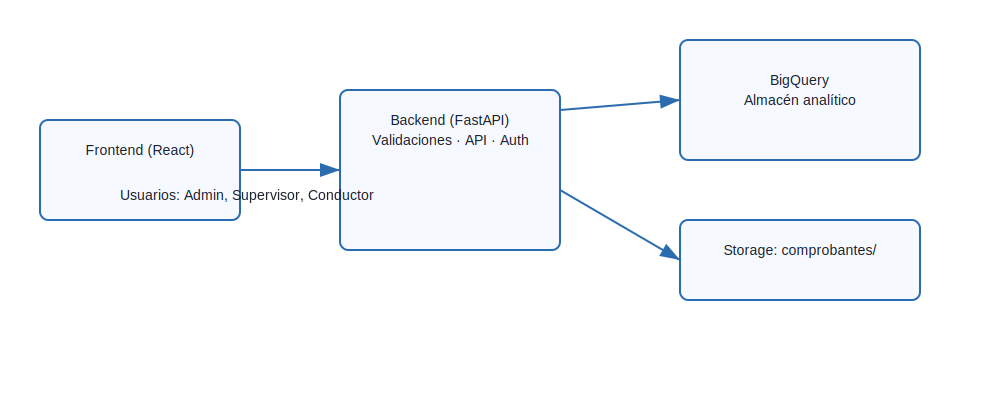
\includegraphics[width=0.9\textwidth]{Images/Project/architecture.pdf}
	\caption{Diagrama de arquitectura general del prototipo XCargo.}
	\label{fig:arquitectura}
\end{figure}

\noindent Referencias sobre frameworks y plataformas utilizados: FastAPI para la construcción de APIs y React para el frontend son soluciones ampliamente adoptadas por su rendimiento y ecosistema \cite{fastapi2020, react2013}.

\section{Modelo de datos y diseño de identificadores}
El diseño del modelo de datos prioriza la trazabilidad: cada registro de pago incluye un identificador de transacción (`Id_Transaccion`), referencia bancaría, fecha/hora, identificador del conductor y punteros a los comprobantes. Para evitar condiciones de carrera en la generación de `Id_Transaccion`, se describe una opción de mejora (uso de UUID o generación centralizada con control de concurrencia) que se evaluará en la fase de pruebas.

\section{Fuentes de datos}
Las fuentes de datos utilizadas durante el prototipo son:
\begin{itemize}
	\item Tablas BigQuery (p. ej. `pagosconductor`, `guias_liquidacion`, `COD_pendientes_v1`).
	\item Archivos de comprobantes almacenados en `backend/comprobantes/`.
	\item Datos de prueba sintetizados para simular escenarios de conciliación y duplicados.
\end{itemize}

\begin{figure}[htbp]
	\centering
	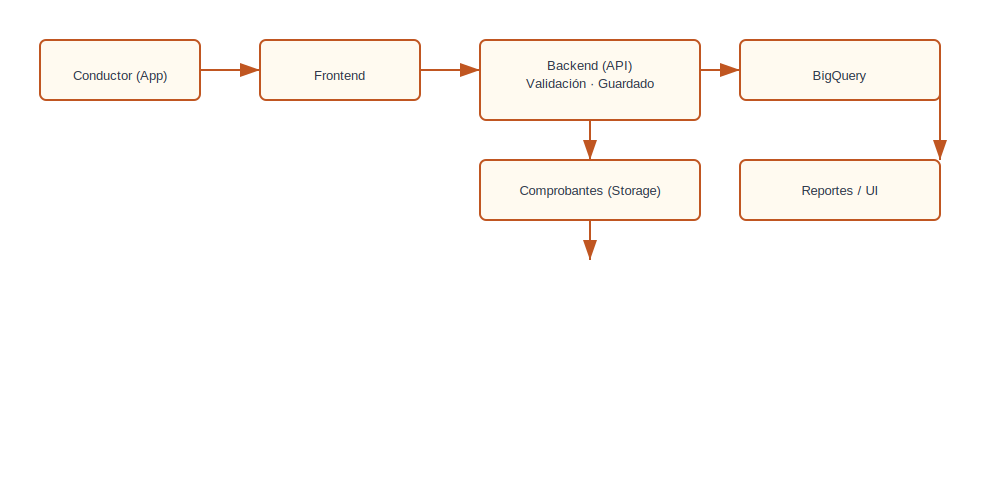
\includegraphics[width=0.85\textwidth]{Images/Project/dataflow.pdf}
	\caption{Flujo de datos: registro de pago, subida de comprobante y conciliación analítica.}
	\label{fig:dataflow}
\end{figure}

\noindent El uso de BigQuery como almacén analítico se documenta ampliamente en la literatura de plataformas en nube y se discuten consideraciones de latencia y coste \cite{bigquery2011}.

\section{Implementación}
La implementación sigue prácticas de desarrollo ágil en ciclos cortos: despliegues locales con `uvicorn --reload` para pruebas rápidas y conjunto de scripts para poblar BigQuery con datos de prueba. Se documentan los endpoints principales y las rutas de uso en el repositorio.

\section{Plan de pruebas y validación}
Las pruebas se estructuran en:
\begin{itemize}
	\item Pruebas unitarias: funciones de validación y utilidades en el backend.
	\item Pruebas de integración: secuencias completas (registro de pago con subida de comprobantes y verificación en BigQuery).
	\item Pruebas funcionales: escenarios reales y edge cases (referencias duplicadas, comprobantes faltantes, formatos incorrectos).
	\item Pruebas de rendimiento: consultas repetidas a BigQuery para estimar latencias y costos por consulta.
\end{itemize}

\section{Métricas de evaluación}
Se definen métricas cuantitativas para evaluar el impacto del prototipo:
\begin{itemize}
	\item Tiempo promedio de conciliación por transacción (antes y después del prototipo).
	\item Tasa de discrepancia (porcentaje de transacciones con errores o duplicados).
	\item Tasa de éxito de conciliación automática (porcentaje de transacciones conciliadas sin intervención manual).
	\item Latencia promedio de consultas analíticas en BigQuery y costo estimado por 1.000 consultas.
\end{itemize}

\section{Consideraciones éticas y de seguridad}
Se incluye el manejo responsable de datos personales (correos, identificadores) y la recomendación de cifrar secretos (mover `SECRET_KEY` a variables de entorno) y restringir el acceso a los comprobantes. En la evaluación se considerarán prácticas de anonimización si se trabaja con datos reales.

\section{Limitaciones}
Se reconocen limitaciones propias del prototipo: uso de almacenamiento local para comprobantes, ausencia de pasarela de pagos integrada y limitaciones de BigQuery como datastore transaccional. Estas restricciones se explican y se proponen líneas de mejora.
